\documentclass{amsart}
\usepackage{amsmath,amsthm,amssymb,IMjournal}
\usepackage{graphicx}
\usepackage{xcolor}

\makeatletter

\newtheorem{thm}{Theorem}[section]
\theoremstyle{definition}
\newtheorem{defn}[thm]{\protect\definitionname}
\theoremstyle{plain}
\newtheorem{prop}[thm]{\protect\propositionname}
\theoremstyle{plain}
\newtheorem{cor}[thm]{\protect\corollaryname}
\theoremstyle{plain}
\newtheorem{rem}[thm]{\protect\remarkname}
\numberwithin{equation}{section}

\makeatother

\providecommand{\corollaryname}{Corollary}
\providecommand{\definitionname}{Definition}
\providecommand{\propositionname}{Proposition}
\providecommand{\remarkname}{Remark}


\begin{document}
\title{Discrete random processes with memory: Models and applications}


\author{\|Tom\'{a}\v{s} |Kou\v{r}im|, \|Petr |Volf|, Prague}


\abstract The contribution focuses on Bernoulli-like random walks
where the past events affect significantly the walk's future
development. The main concern of the paper is therefore the
formulation of models describing the dependence of transition
probabilities on the process history. Such an impact can be
incorporated explicitly and transition probabilities modulated
using a few parameters reflecting the current state of the walk as
well as the information about the past path. The behavior of
proposed random walks, as well as the task of their parameters
estimation, are studied both theoretically and with the aid of
simulations.
\endabstract

\keywords
 Random walk, history dependent transition
probabilities, non-Markov process, success punishing/rewarding walk
\endkeywords

\subjclass
60G50, 62F10
\endsubjclass

\thanks
The research was supported by the grant No. 18-02739S of the Grant
Agency of the Czech Republic.
\endthanks

\section{Introduction}
One of the most
common types of a discrete random process is a random walk,
first introduced by K.Pearson in 1905 \cite{pearson1905problem}.
There exist many
variations of a random walk with various applications to real life
problems \cite{schutz2004elephants,turban2010random}. Yet there are
still new possibilities and options how to alter and improve the classical
random walk and present yet another model representing different real
life events. One of such modifications is the random walk with varying
step size introduced in $2010$ by Turban \cite{turban2010random}
which, together with the idea of \emph{self-exciting point processes}
\cite{hawkes1971spectra} and the perspective of model applications
in reliability analysis and also in sports statistics, served as an
inspiration to the random walk with varying transition probabilities
introduced by Kou\v{r}im \cite{ja2017ddny, ja2019teze}. The definition of the walk falls into a rather broad class of processes described for instance in the paper of
Davis and Liu \cite{davis2012theory}. However, other assumptions, e.g. the condition of contraction, are
not fulfilled by the walk and thus the conclusions from  \cite{davis2012theory} cannot be applied.

In the present paper, the theoretical properties of the model are
described and further examined, numerical procedures of model
parameters estimation are specified and the results are tested on
generated data.

The rest of the paper is organized as follows. Sections
\ref{sec:Random-walk-with} and \ref{sec:Random-walk-aternatives}
describe the properties of different versions of the model,
section \ref{sec:Simulations} provides results from simulated
model {\color{red}evaluation} and finally section \ref{sec:Conclusion} concludes
the work.

\section{Random walk with varying probabilities\label{sec:Random-walk-with}}

The random walk with varying probabilities is based on a standard
Bernoulli random walk \cite{feller1957introduction} with some starting
transition probability $p_{0}$. This probability is then altered
after each step of the walk using a coefficient $\lambda$ so that
the repetition of the same step becomes less probable. Formally, it
can be defined as
\begin{defn}
\label{success_punished}Let ${\{X_{n}\}}_{n=1}^{\infty}$ and ${\{P_{n}\}}_{n=1}^{\infty}$
be sequences of discrete random variables, and $p_{0}\in[0,\,1]$
and $\lambda\in(0,\,1)$ constant parameters, such that the first
random variable $X_{1}$ is given by
\[
P(X_{1}=1)=p_{0},\,\,\,
P(X_{1}=-1)=1-p_{0}.
\]
Further
\begin{equation}
P_{1}=\lambda p_{0}+\frac{1}{2}(1-\lambda)(1-X_{1})\label{eq:P!1_def}
\end{equation}
and for $i\geq2$
\[
P(X_{i}=1|P_{i-1}=p_{i-1})=p_{i-1},\,\,\,
P(X_{i}=-1|P_{i-1}=p_{i-1})=1-p_{i-1},
\]
\begin{equation}
P_{i}=\lambda P_{i-1}+\frac{1}{2}(1-\lambda)(1-X_{i}).\label{eq:Pi_def}
\end{equation}
The sequence ${\{S_{n}\}}{}_{n=0}^{\infty},\;S_{N}=S_{0}+\sum_{i=1}^{N}X_{i}$
for $n\in\mathbb{N}$, with $S_{0}\in\mathbb{R}$ some given starting
position, is called a \emph{random walk with varying probabilities},
with ${\{X_{n}\}}_{n=1}^{\infty}$ being the steps of the walker and
${\{P_{n}\}}_{n=1}^{\infty}$ transition probabilities.
\end{defn}

\subsection{Properties}

The random walk with varying probabilities was first introduced in
\cite{ja2017ddny} and further elaborated in \cite{ja2019teze}.
Following properties of the walk were described in these previous
papers.

The value of a transition probability $P_{t+k}$ at
each step $t+k,\;t,\,k>0$ can be computed from the knowledge of
transition probability $P_{t}$ and the realization of the walk
$X_{t+1},\,\dots,\,X_{t+k}$ using formula
\begin{equation}
P_{t+k}=P_{t}\lambda^{k}+\frac{1}{2}(1-\lambda)\sum_{i=t+1}^{t+k}\lambda^{t+k-i}(1-X_{i}).\label{eq:Pt}
\end{equation} 
To compute the expected value of transition probability and position of the walker following formula can be used
\begin{equation}
EP_{t}=(2\lambda-1)^{t}p_{0}+\frac{1-(2\lambda-1)^{t}}{2}\label{eq:EPt}
\end{equation}
and
\begin{equation}
ES_{t}=S_{0}+(2p_{0}-1)\frac{1-(2\lambda-1)^{t}}{2(1-\lambda)}\label{eq:ESt}
\end{equation}
 for all $t\geq1$. This further yields $EP_{t}\rightarrow\frac{1}{2}$
and $ES_{t}\rightarrow S_{0}+\frac{2p_{0}-1}{2(1-\lambda)}$ for $t\rightarrow+\infty$.

Now to describe the walk in more detail, let us
prove the following propositions.

\begin{prop}\label{PropEXt-succes}
For all $t\geq1,$ it holds that
\begin{equation}
E(X_{t})=(2\lambda-1)^{t-1}(2p_{0}-1).
\end{equation}
\end{prop}
\begin{proof}
Using that $E(X_{t})=2P_{t-1}-1$ the proposition can be
proved directly using \eqref{eq:EPt} as
\[
E(X_{t})=E(E(X_{t})|X_{t-1})=E(2P_{t-1}-1)=2E(P_{t-1})-1=
\]
\[
=2((2\lambda-1)^{t-1}p_{0}+\frac{1-(2\lambda-1)^{t-1}}{2})-1=(2\lambda-1)^{t-1}(2p_{0}-1).
\]
\end{proof}

\begin{cor}
\label{cor-stac-dist}
The distribution of $X_t$ converges to the Bernoulli $(1,\,-1)$ distribution with
$p=\frac{1}{2}$. This Bernoulli distribution is simultaneously the stationary distribution of the random sequence $X_t$.
\end{cor}

\begin{proof}
As $X_t$ are Bernoulli $(1,\,-1)$, their distributions are fully characterized by their expectations $EX_t$, and it holds that
$EX_t=2\cdot EP_{t-1}-1$. Then the first statement of the Corollary follows from the fact that $EP_t\to \frac{1}{2}.$

Further, let $EP_{t-1}=\frac{1}{2}$ be the characteristics of $X_t$, i.e.
$EX_t=0$. As then
$EP_t=EP_{t-1}\lambda+(1-\lambda)/2(1-EX_t)=\frac{1}{2}$, therefore $EX_{t+1}=0$ again.

\end{proof}

\begin{rem}
For $p_0=\frac{1}{2}$ and $t\ge1$ or $\lambda = \frac{1}{2}$ and $t\ge2$ it hods that $X_t$ is the stationary
random sequence with the distribution given by Corollary
\ref{cor-stac-dist}.
\end{rem}

\begin{prop}
\label{PropVarP-succes}For all $t\geq1,$ it holds that
\begin{equation}
Var(P_{t})=(3\lambda^{2}-2\lambda)^{t}p_{0}^{2}+\sum_{i=1}^{t}K(i-1)(3\lambda^{2}-2\lambda)^{t-i}-k(t)^{2},\label{eq:VarP-proposition}
\end{equation}
 where
\[
k(t)=EP_{t}=(2\lambda-1)^{t}p_{0}+\frac{1-(2\lambda-1)^{t}}{2}
\]
 and
\[
K(t)=k(t)\cdot(-3\lambda^{2}+4\lambda-1)+(1-\lambda)^{2}.
\]
\end{prop}

\begin{proof}
To prove the proposition several support formulas has to be derived
first. From the definition of variance it follows
\begin{equation}
Var(P_{t})=E(P_{t}^{2})-E(P_{t})^{2}.\label{eq:VarP-definition}
\end{equation}
$E(P_{t})$ is given by (\ref{eq:EPt}), therefore in order to prove
the proposition it is sufficient to prove the following statement
\begin{equation}
E(P_{t}^{2})=(3\lambda^{2}-2\lambda)^{t}p_{0}^{2}+\sum_{i=1}^{t}K(i-1)(3\lambda^{2}-2\lambda)^{t-i}.\label{eq:EPt2-finalvzorec}
\end{equation}
To do so, let us first express the relation between $E(P_{t}^{2})$
and $E(P_{t-1}^{2})$ and $E(P_{t-1}).$ From the definition of the
expected value and the definition of the walk (\ref{eq:Pi_def}) it follows
\begin{equation}
E(P_{t}^{2})=E[E(P_{t}^{2}|P_{t-1})]=E[E(\lambda P_{t-1}+\frac{1}{2}(1-\lambda)(1-X_{t}))^{2}|P_{t-1}].\label{eq:EPt2-zaklad}
\end{equation}
Using that $E(X_{t}|P_{t-1})=2P_{t-1}-1$, $E(X_{t}^{2})=1$ and further
that
\[
E[(1-X_{t})^{2}|P_{t-1}]=E[(1-2X_{t}+X_{t}^{2})|P_{t-1}]
=E[(2-2X_{t})|P_{t-1}]= 4(1-P_{t-1}).
\]
Equation (\ref{eq:EPt2-zaklad}) further yields
\[
E(P_{t}^{2})=E[\lambda^{2}P_{t-1}^{2}+\lambda P_{t-1}(1-\lambda)E(1-X_{t}|P_{t-1})+\frac{1}{4}(1-\lambda)^{2}E((1-X_{t})^{2}|P_{t-1})]=
\]
\[
=E[\lambda^{2}P_{t-1}^{2}+2\lambda P_{t-1}(1-\lambda)(1-P_{t-1})+(1-\lambda)^{2}(1-P_{t-1})]
\]
 and finally
\begin{equation}
E(P_{t}^{2})=E(P_{t-1}^{2})(3\lambda^{2}-2\lambda)+EP_{t-1}(-3\lambda^{2}+4\lambda-1)+(1-\lambda)^{2}.\label{eq:EPt2-pokrocile}
\end{equation}
Statement (\ref{eq:EPt2-finalvzorec}) can be proved using mathematical induction.
Based on the trivial fact that $Ep_{0}=p_{0}$ and $E(p_{0})^{2}=p_{0}^{2}$,
for $t=1$ we get
\[
E(P_{1}^{2})=(3\lambda^{2}-2\lambda)^{1}p_{0}^{2}+\sum_{i=1}^{1}K(i-1)(3\lambda^{2}-2\lambda)^{1-i}=(3\lambda^{2}-2\lambda)p_{0}^{2}+K(0)=
\]
\[
=(3\lambda^{2}-2\lambda)p_{0}^{2}+((2\lambda-1)^{0}p_{0}+\frac{1-(2\lambda-1)^{0}}{2})\cdot(-3\lambda^{2}+4\lambda-1)+(1-\lambda)^{2}=
\]
\[
=(3\lambda^{2}-2\lambda)p_{0}^{2}+p_{0}(-3\lambda^{2}+4\lambda-1)+(1-\lambda)^{2},
\]
and from (\ref{eq:EPt2-pokrocile}) it follows that \eqref{eq:EPt2-finalvzorec}
holds for $t=1$. Now for the induction step $t\rightarrow t+1$ we get by substituting
(\ref{eq:EPt2-finalvzorec}) into (\ref{eq:EPt2-pokrocile})
\[
E(P_{t+1}^{2})=E(P_{t}^{2})(3\lambda^{2}-2\lambda)+EP_{t}(-3\lambda^{2}+4\lambda-1)+(1-\lambda)^{2}=
\]
\[
=((3\lambda^{2}-2\lambda)^{t}p_{0}^{2}+\sum_{i=1}^{t}K(i-1)(3\lambda^{2}-2\lambda)^{t-i})\cdot(3\lambda^{2}-2\lambda)+K(t)=
\]
\[
=(3\lambda^{2}-2\lambda)^{t+1}p_{0}^{2}+\sum_{i=1}^{t}K(i-1)(3\lambda^{2}-2\lambda)^{t+1-i}+K(t)=
\]
\[
=(3\lambda^{2}-2\lambda)^{t+1}p_{0}^{2}+\sum_{i=1}^{t+1}K(i-1)(3\lambda^{2}-2\lambda)^{t+1-i}
\]
and the formula thus holds. Now substituting (\ref{eq:EPt}) and (\ref{eq:EPt2-finalvzorec})
into (\ref{eq:VarP-definition}) yields (\ref{eq:VarP-proposition})
and proves the Proposition.
\end{proof}
From Proposition \ref{PropVarP-succes} the limit behavior of $Var(P_{t})$
can be derived easily:

\begin{cor}
For $t\rightarrow+\infty,$ \textup{
\begin{equation}
\lim_{t\to+\infty}Var(P_{t})=\frac{\frac{1}{2}(1-\lambda^{2})}{1-3\lambda^{2}+2\lambda}-\frac{1}{4}.\label{eq:CoroVarpt-statement}
\end{equation}
}
\end{cor}

Figure \ref{fig:The-development-punished} shows the comparison of
computed theoretical values of transition probability expected value and its variance and the actual observed values of average transition
probability and variance for different starting probabilities $p_{0}$
and memory coefficients $\lambda$.


\begin{prop}\label{propVarX}
For all $t\geq1,$ it holds that
\begin{equation}
Var(X_{t})=1-(2\lambda-1)^{2(t-1)}(2p_{0}-1)^2.
\end{equation}
\end{prop}
\begin{proof}
The fact that $X_t$ are Bernoulli $(1,\,-1)$ implies $E(X_{t}^2)=1$. The statement then follows directly from the definition of variance and Proposition \ref{PropEXt-succes}.
\end{proof}


\begin{cor}
For $t\rightarrow+\infty,$ \textup{
\begin{equation}
\lim_{t\to+\infty}Var(X_{t})=1.
\end{equation}
}
\end{cor}

The variance of the position of the walker was studied with the help of computer simulations, presented in Figure \ref{fig:position-punished}. The simulations show that the variance grows to infinity with $t\rightarrow\infty$ depending on both $p_0$ and $\lambda$. The derivation of an exact formula will be subject of further studies.

\begin{figure}
 \begin{center}
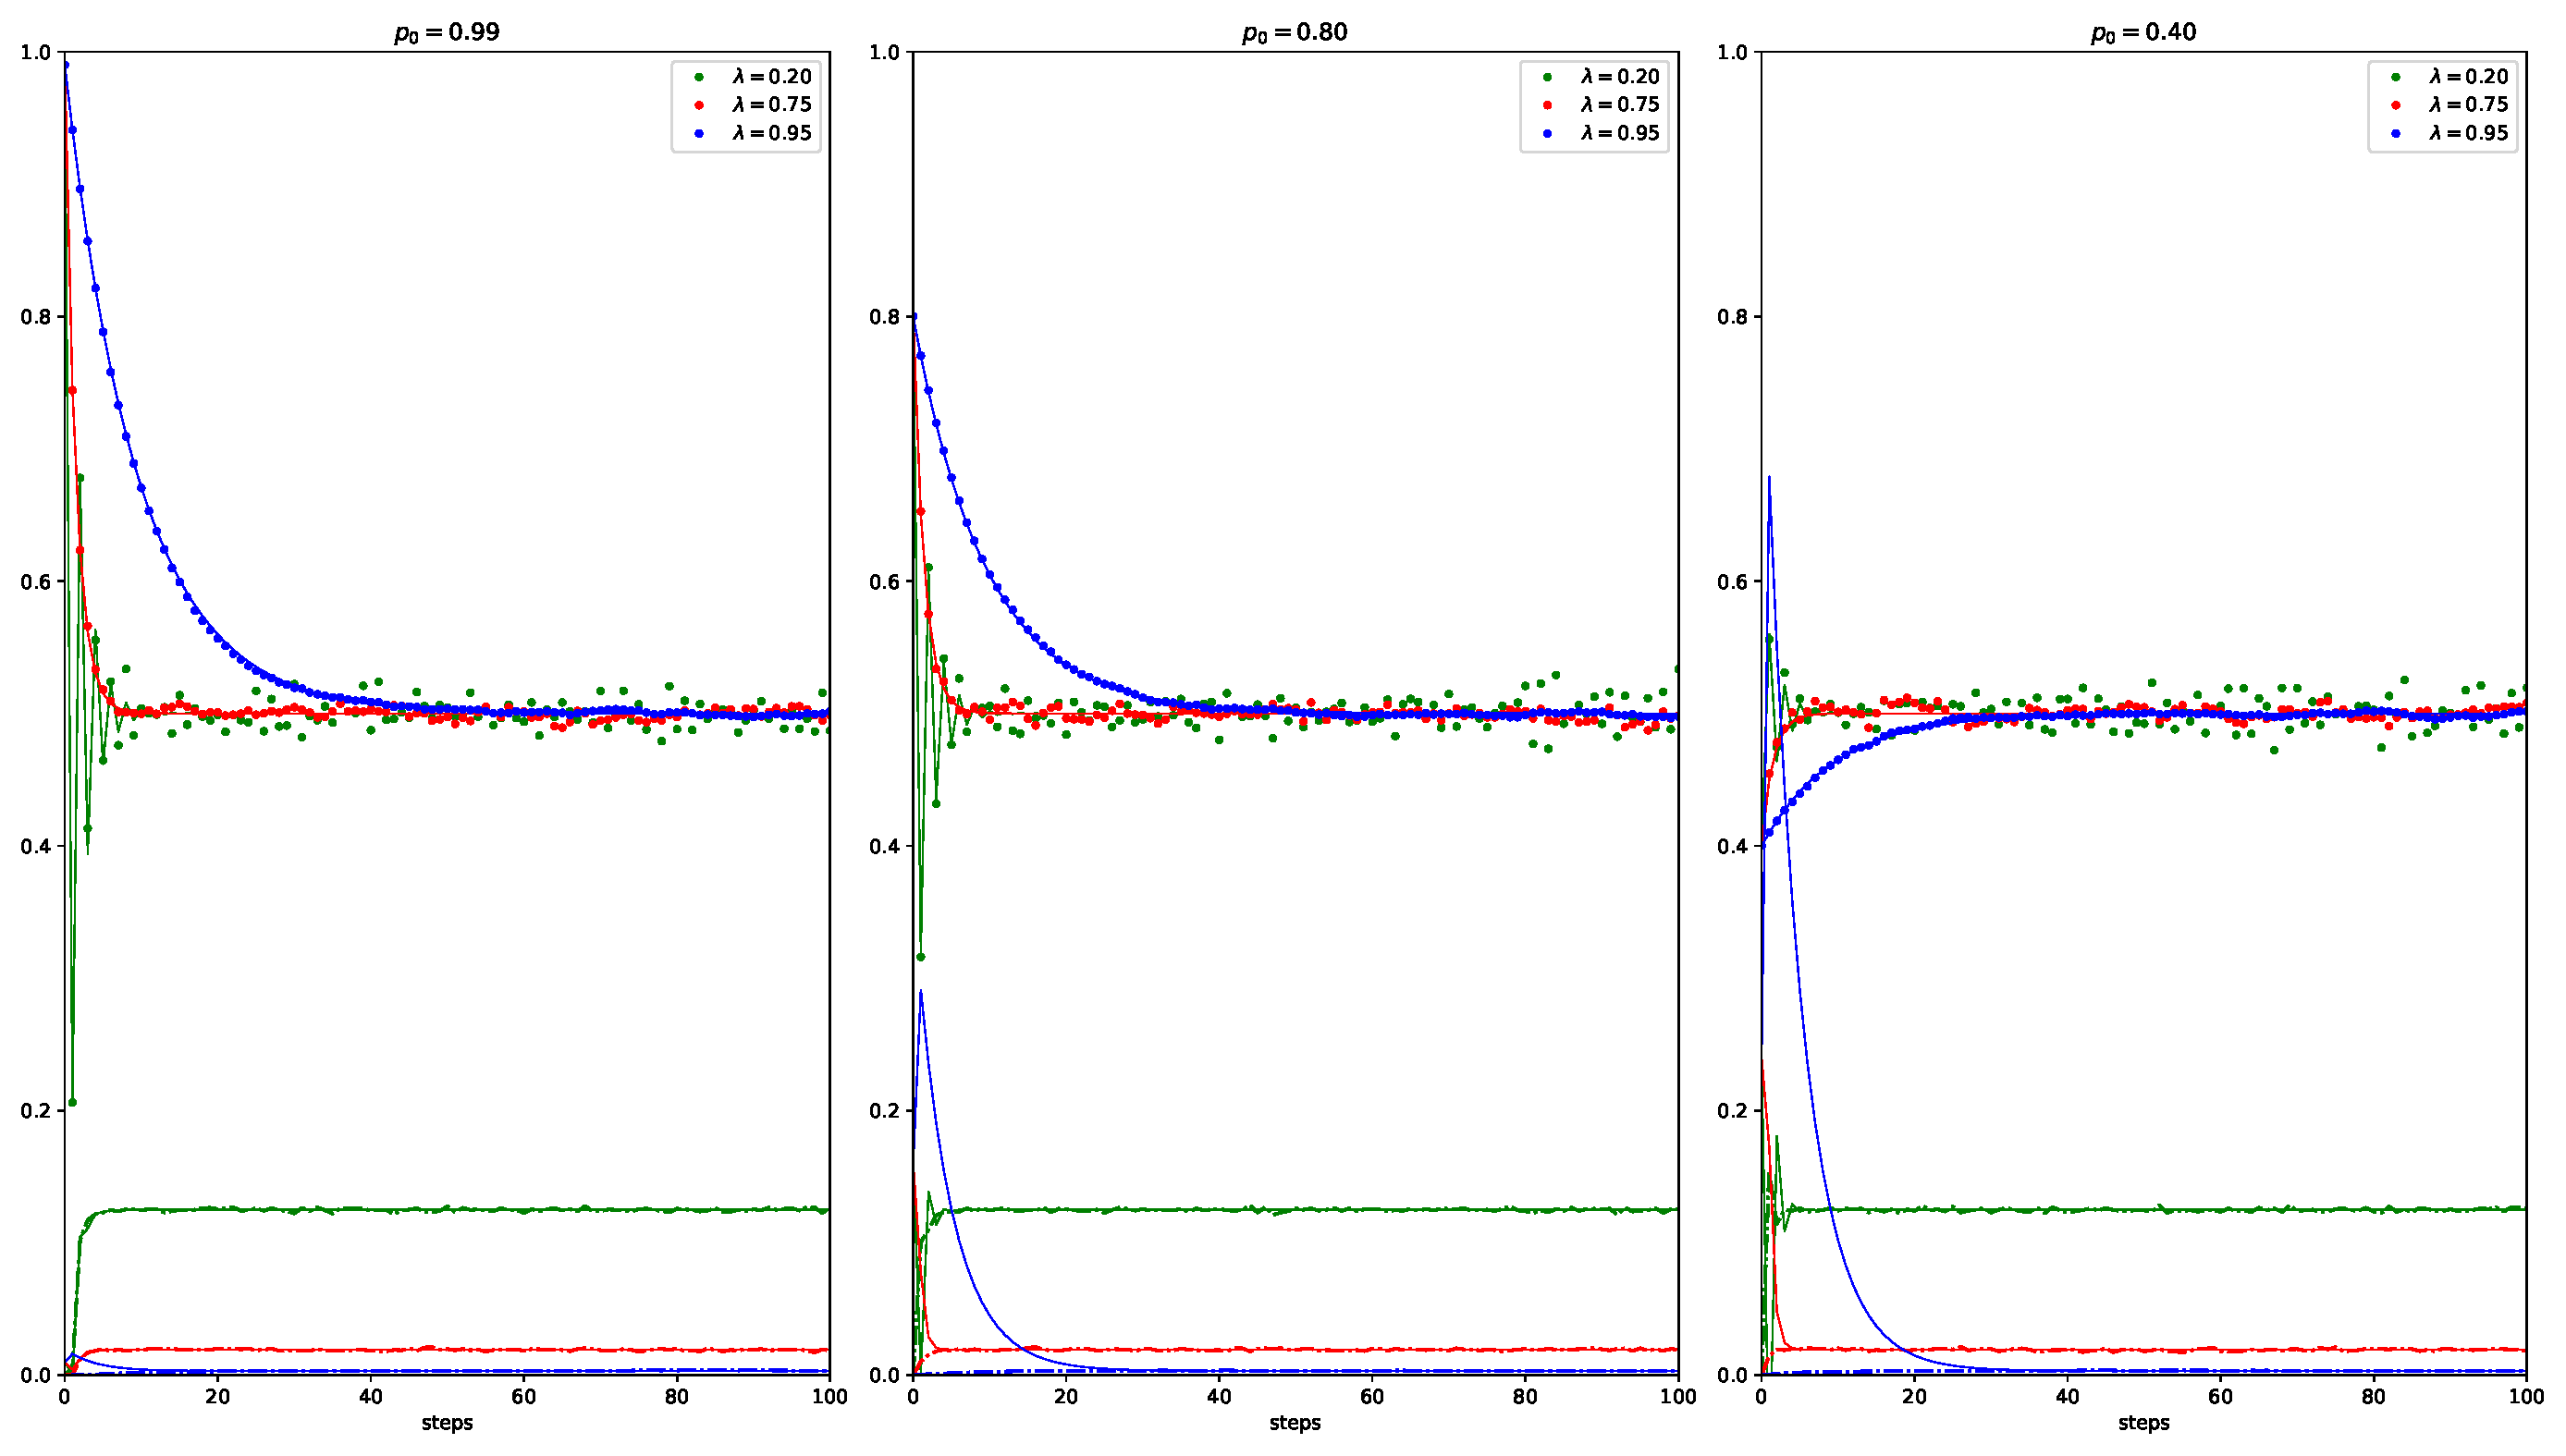
\includegraphics[width=1\textwidth]{../simulations/e_probability_1000_walks_100_steps_type_success_punished}
\caption{\label{fig:The-development-punished}The observed
average transition probability (dotted, upper part of the figure)
of a \emph{success punishing} version of the random walk and its observed
variance (dot-dashed lines, lower part of the figure) compared to
the theoretical values computed using (\ref{eq:EPt}) and Proposition
\ref{PropVarP-succes} (same colors, solid lines). The values were
computed from 1000 simulated realizations of each parameter combination.}
 \end{center}
\end{figure}

\begin{figure}
 \begin{center}
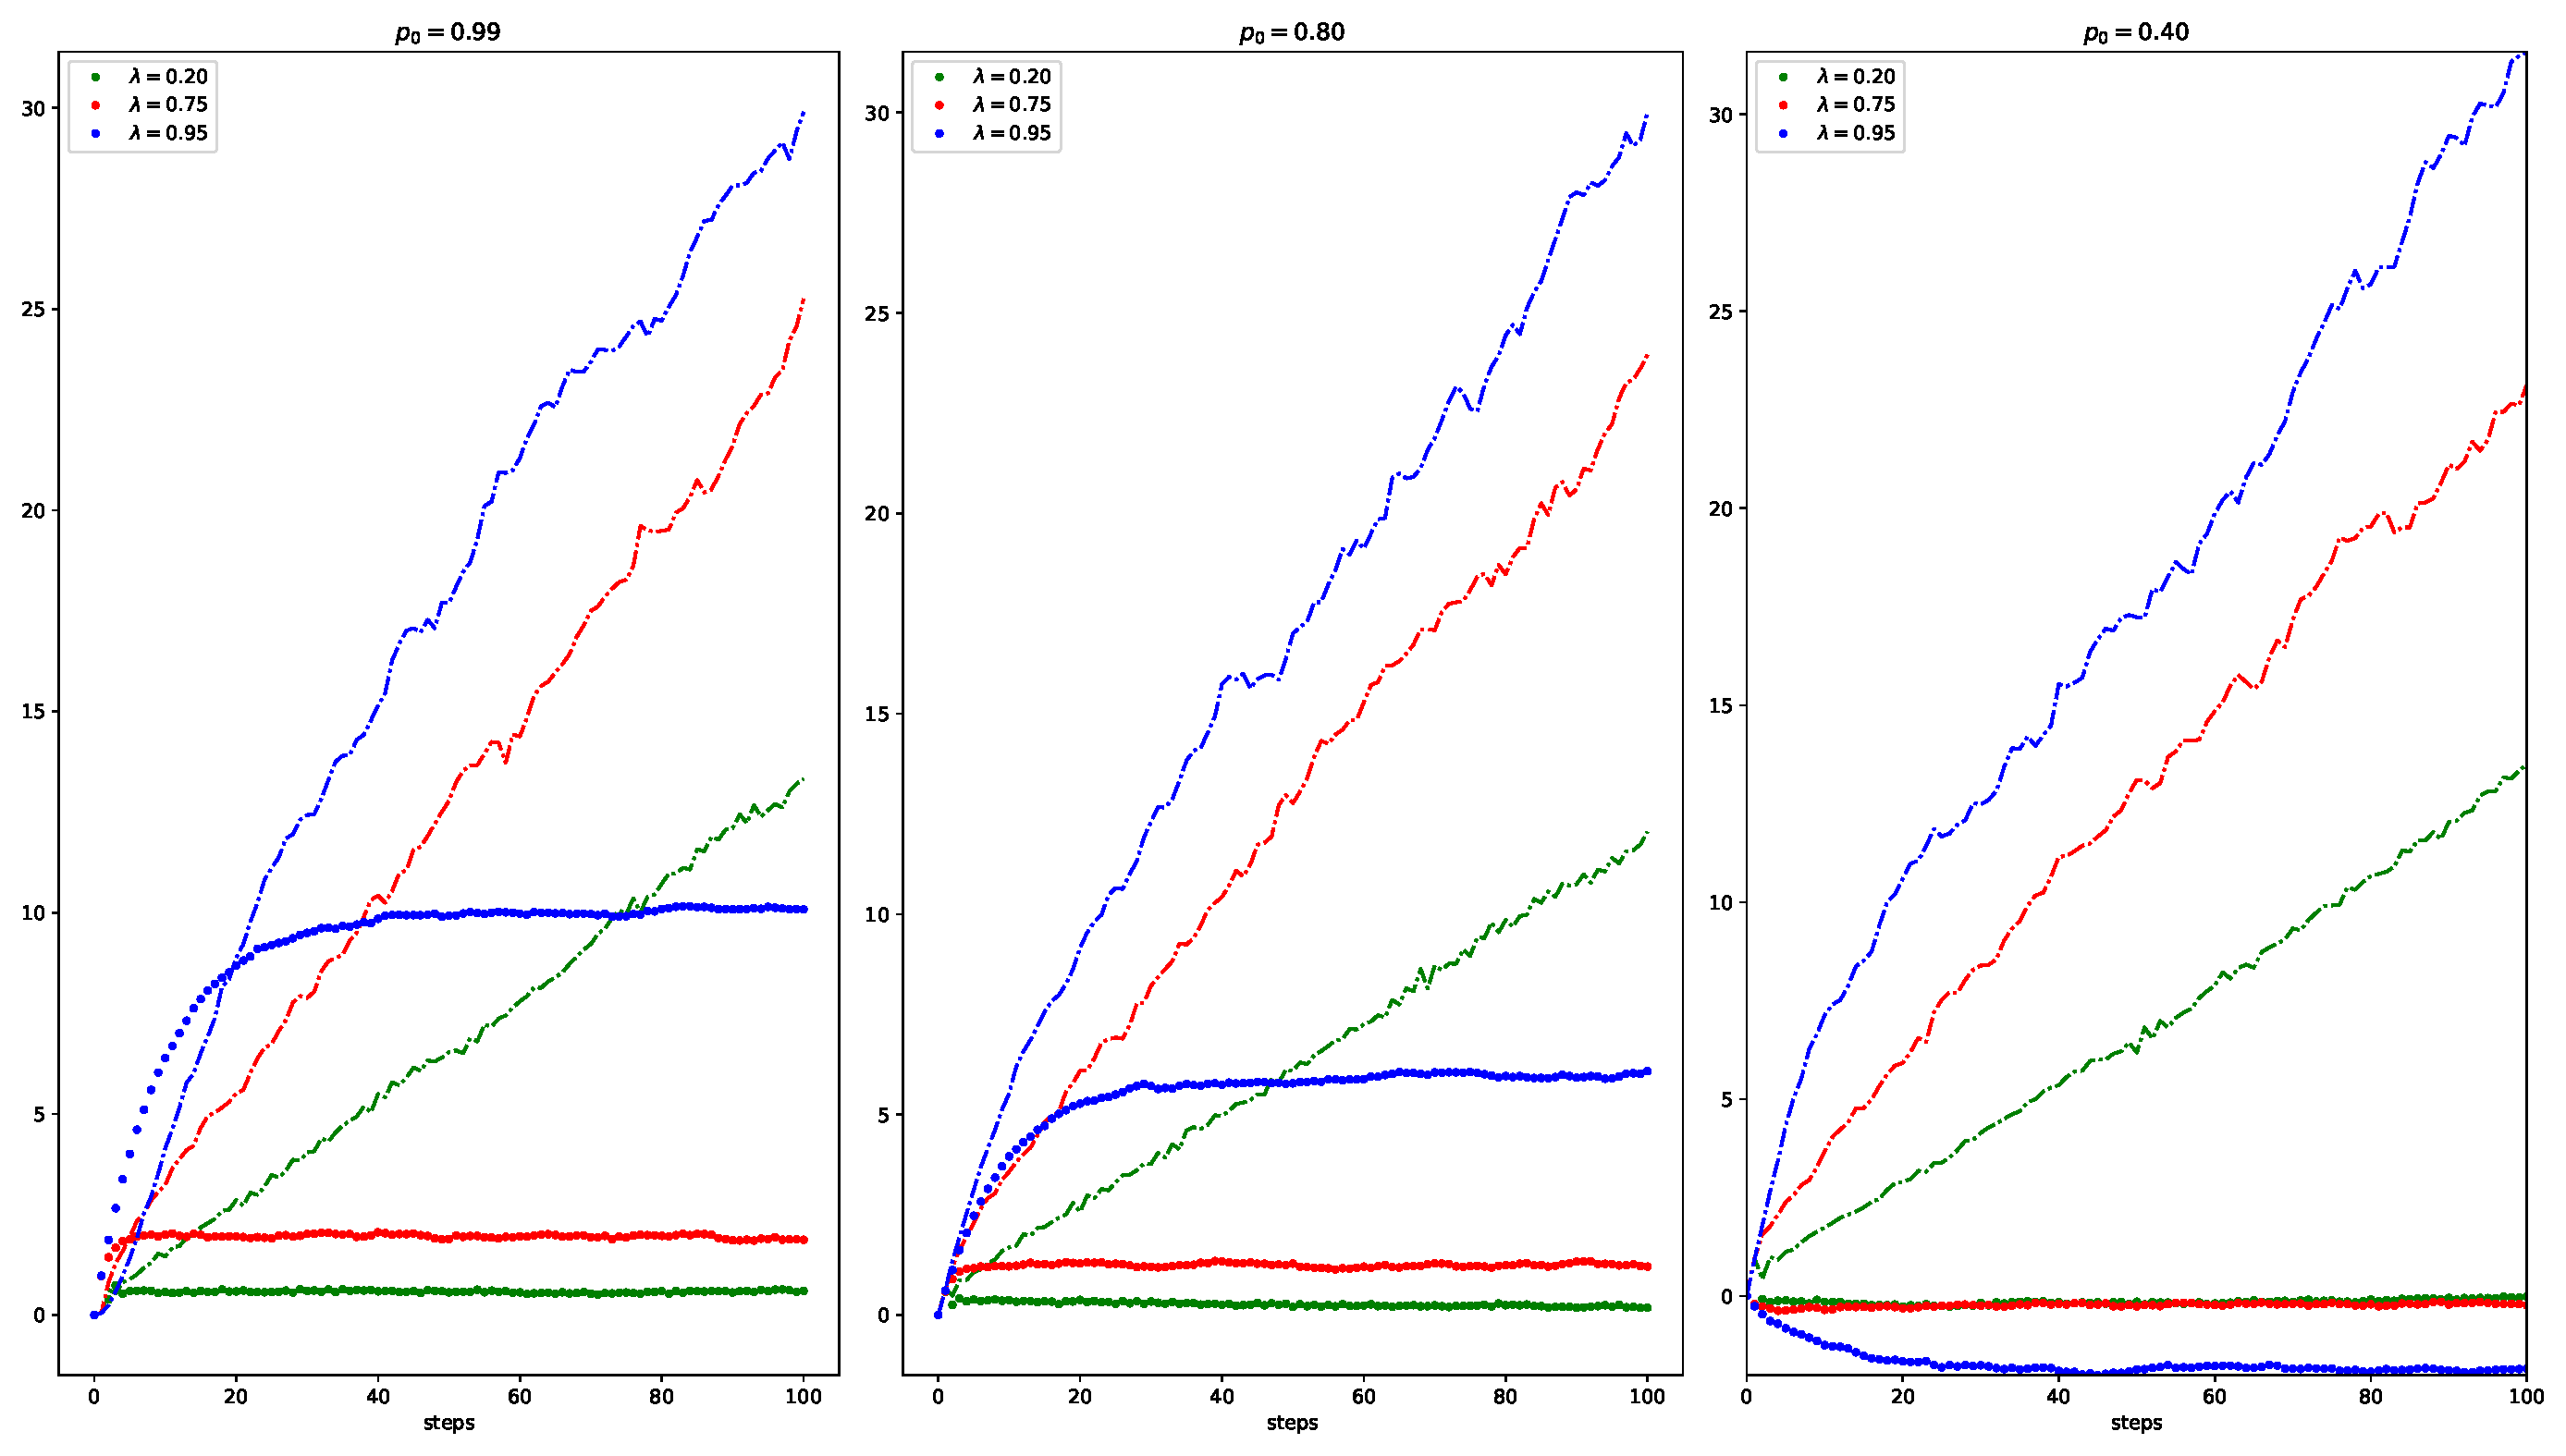
\includegraphics[width=1\textwidth]{../simulations/e_position_1000_walks_100_steps_type_success_punished}
\caption{\label{fig:position-punished}The observed
average position of the walker (dotted, ``thicker'')
of a \emph{success punishing} version of the random walk and its variance (dot-dashed lines, ``thinner''). The values were
computed from 1000 simulated realizations of each parameter combination.}
 \end{center}
\end{figure}


\section{Random walk with varying transition probability - alternatives\label{sec:Random-walk-aternatives}}

\subsection{Success rewarding model}

The basic definition of the random walk (Definition \ref{success_punished})
presents a \emph{success punishing} model, meaning that the probability
of an event is decreased every time that event occurs. Opposite situation
can be considered, where the probability of an event is increased
with each event's occurrence. Formally, such a random walk is defined
in a following manner \cite{ja2019teze}:

\begin{defn}
\label{succes_rewarded}Let ${\{X_{n}\}}_{n=1}^{\infty}$, $p_{0}$
and $\lambda$ be as in Definition \ref{success_punished}. Further
let ${\{P_{n}\}}_{n=1}^{\infty}$ be a sequence of discrete random
variables given by
\begin{equation}
P_{1}=\lambda p_{0}+\frac{1}{2}(1-\lambda)(1+X_{1}),\label{eq:P1_def-reward}
\end{equation}
\begin{equation}
P_{i}=\lambda P_{i-1}+\frac{1}{2}(1-\lambda)(1+X_{i})\;\;\forall i\geq2.\label{eq:Pi_def-reward}
\end{equation}

The sequence ${\{S_{n}\}}{}_{n=0}^{\infty},$ given as in Definition \ref{success_punished}, is a random walk with varying probabilities - \emph{success
rewarding}.
\end{defn}
In this section, all variables ($P,\,X,\,S$) are related to the
\emph{success rewarding} model. This version of the model behaves differently
than the \emph{success punishing} version, which can be observed with
the help of the following propositions.

\begin{prop}
For all $t\ge 2,$
\begin{equation}
P_{t}=p_{0}\lambda^{t}+\frac{1}{2}(1-\lambda)\sum_{i=1}^{t}\lambda^{t-i}(1+X_{i}).\label{eq:propSuccess1}
\end{equation}
\end{prop}

\begin{proof}
The Proposition is proved using mathematical induction. For $t=2$ using (\ref{eq:P1_def-reward})
and (\ref{eq:Pi_def-reward}) it holds that
\[
P_{2}=\lambda P_{1}+\frac{1}{2}(1-\lambda)(1+X_{2})=\lambda(\lambda p_{0}+\frac{1}{2}(1-\lambda)(1+X_{1}))+\frac{1}{2}(1-\lambda)(1+X_{2})=
\]

\[
=p_{0}\lambda^{2}+\frac{1}{2}(1-\lambda)\sum_{i=1}^{2}\lambda^{2-i}(1+X_{i}),
\]
which is in accordance with (\ref{eq:propSuccess1}). Now for the
induction step $t\rightarrow t+1$ we obtain from (\ref{eq:Pi_def-reward})
and the induction assumption
\[
P_{t+1}=\lambda P_{t}+\frac{1}{2}(1-\lambda)(1+X_{t+1})=
\]
\[
=\lambda(p_{0}\lambda^{t}+\frac{1}{2}(1-\lambda)\sum_{i=1}^{t}\lambda^{t-i}(1+X_{i}))+\frac{1}{2}(1-\lambda)(1+X_{t+1})=
\]
\[
=p_{0}\lambda^{t+1}+\frac{1}{2}(1-\lambda)\sum_{i=1}^{t}\lambda^{t-i+1}(1+X_{i})+\frac{1}{2}(1-\lambda)(1+X_{t+1})=
\]
\[
=p_{0}\lambda^{t+1}+\frac{1}{2}(1-\lambda)\sum_{i=1}^{t+1}\lambda^{t+1-i}(1+X_{i}).
\]
\end{proof}

\begin{prop}
\label{PropReward2}For all $t\geq1,$ $E(P_{t})=p_{0}.$
\end{prop}
\begin{proof}
Using $E(X_{t}|P_{t-1})=2P_{t-1}-1$ and (\ref{eq:Pi_def-reward})
we obtain
\[
EP_{t}=E[E(P_{t}|P_{t-1})]=E[E(\lambda P_{t-1}+\frac{1}{2}(1-\lambda)(1+X_{t})|P_{t-1})]=
\]
\[
=E[\lambda P_{t-1}+\frac{1}{2}(1-\lambda)(1+2P_{t-1}-1)]=E[\lambda P_{t-1}+(1-\lambda)P_{t-1})=  E(P_{t-1}).
\]
Recursively we get
\begin{equation}
E(P_{t})=E(p_{0})=p_{0}.\label{eq:EPt-reward-formula}
\end{equation}
\end{proof}

\begin{prop}
The sequence $X_t$ is a stationary sequence of Bernoulli random
variables with values $1,\,-1$ and with $P(X_t=1)=p_0$.
\end{prop}
\begin{proof}
As the distribution of $X_t$ is fully given by $E(P_{t-1})$, the
statement follows directly from Proposition \ref{PropReward2}.
\end{proof}

\begin{prop}
Bernoulli $(0,\,1)$ distribution with parameter $q$ is  {\color{red}a} stationary distribution of the random sequence
${\{P_{t}\}}_{t=1}^{\infty}$.
\end{prop}
\begin{proof}
Let $P_{t-1}=1$ with probability $q$, then $X_t=1$, or
$P_{t-1}=0$ with $1-q$, then $X_t=-1$.  From \eqref{eq:Pi_def-reward} it follows that with probability
$q$ $P_t=\lambda\cdot 1+(1-\lambda)\cdot 2/2=1$, while with
probability $1-q$ $P_t=\lambda\cdot 0+(1-\lambda)\cdot 0/2=0$.
It means that $P_t$ has the same Bernoulli distribution as
$P_{t-1}$.
\end{proof}

Now to calculate the expected position of the walker at a given
step $t\geq1$, {\color{red} the definition of the walk can be used to to prove that $E(X_{t}|S_{t-1})=E(X_{t}|P_{t-1}) = 2P_{t-1}-1$ and thus}
$E(S_{t}{\color{red}|S_{t-1}})=S_{t-1}+2P_{t-1}-1$. From this, we can prove the
following statement about the expected position of the walker
after step $t$ just from the knowledge of the input parameters.

\begin{prop}
For all $t\geq1,$
\[
E(S_{t})=S_{0}+t(2p_{0}-1).
\]
\end{prop}
\begin{proof}
Using the result of Proposition \ref{PropReward2} we get
\[
E(S_{t+1})=E[E(S_{t+1}|S_{t})]=E[S_{t}+(2P_{ \color{red}t}-1)]=
ES_{t}+(2p_{0}-1)
\]

which then recursively proves the statement.
\end{proof}

\begin{cor}
For $t\rightarrow+\infty,$ \textup{
\[
\lim_{t\to+\infty}E(S_{t})=\begin{cases}
+\infty & p_{0}>\frac{1}{2}\\
0 & p_{0}=\frac{1}{2}\\
-\infty & p_{0}<\frac{1}{2}
\end{cases}.
\]
}
\end{cor}

\begin{prop}
For all $t\geq1,$
\begin{equation}
Var(P_{t})=(2\lambda-\lambda^{2})^{t}p_{0}^{2}+p_{0}(1-\lambda)^{2}\sum_{i=1}^{t}(2\lambda-\lambda^{2})^{t-i}-p_{0}^{2}.\label{eq:VarPt-reward-prop}
\end{equation}
\end{prop}
\begin{proof}
The proof will be done in several steps similar as in Proposition
\ref{PropVarP-succes}. It is based on the definition of variance \eqref{eq:VarP-definition}. From Proposition \ref{PropReward2} it follows $E(P_{t})=p_{0}$ and
it is thus sufficient to prove that
\begin{equation}
E(P_{t}^{2})=(2\lambda-\lambda^{2})^{t}p_{0}^{2}+p_{0}(1-\lambda)^{2}\sum_{i=1}^{t}(2\lambda-\lambda^{2})^{t-i}.\label{eq:Ept2-finalvzorec-reward}
\end{equation}
The proof will be done using mathematical induction again. First observe that
\[
E(P_{t}^{2})=E[E(P_{t}^{2}|P_{t-1})]=E[E(\lambda P_{t-1}+\frac{1}{2}(1-\lambda)(1+X_{t}))^{2}|P_{t-1}]=
\]
\begin{equation}
=EP_{t-1}^{2}(2\lambda-\lambda^{2})+p_{0}(1-\lambda)^{2},\label{eq:EPt-EPt-1-reward}
\end{equation}
where the facts that $E[(1+X_{t})^{2}|P_{t-1}]=4P_{t-1}$, $E[(1+X_{t})|P_{t-1}]=2P_{t-1}$
and Proposition \ref{PropReward2} were used. Now for $t=1$ we get
\[
EP_{1}=p_{0}^{2}(2\lambda-\lambda^{2})+p_{0}(1-\lambda)^{2}=(2\lambda-\lambda^{2})^{1}p_{0}^{2}+p_{0}(1-\lambda)^{2}\sum_{i=1}^{1}(2\lambda-\lambda^{2})^{1-i}
\]
and thus \eqref{eq:Ept2-finalvzorec-reward} holds for $t=1$. For the induction step $t\rightarrow t+1$
we get from the induction assumption and (\ref{eq:EPt-EPt-1-reward})
\[
E(P_{t+1}^{2})=EP_{t}^{2}(2\lambda-\lambda^{2})+p_{0}(1-\lambda)^{2}=
\]
\[
=((2\lambda-\lambda^{2})^{t}p_{0}^{2}+p_{0}(1-\lambda)^{2}\sum_{i=1}^{t}(2\lambda-\lambda^{2})^{t-i})\cdot(2\lambda-\lambda^{2})+p_{0}(1-\lambda)^{2}=
\]

\[
=(2\lambda-\lambda^{2})^{t+1}p_{0}^{2}+p_{0}(1-\lambda)^{2}\sum_{i=1}^{t}(2\lambda-\lambda^{2})^{t-i+1}+p_{0}(1-\lambda)^{2}=
\]
\[
=(2\lambda-\lambda^{2})^{t+1}p_{0}^{2}+p_{0}(1-\lambda)^{2}\sum_{i=1}^{t+1}(2\lambda-\lambda^{2})^{t+1-i}.
\]
The Proposition is then proved by substituting (\ref{eq:EPt-reward-formula})
and (\ref{eq:Ept2-finalvzorec-reward}) into \eqref{eq:VarP-definition}.
\end{proof}
Notice that the last sum in (\ref{eq:VarPt-reward-prop}), after re-indexing
by $j=t-i$, yields 
\[
\sum_{j=0}^{t-1}(2\lambda-\lambda^{2})^{j}=\frac{1-(2\lambda-\lambda^{2})^{t}}{1-2\lambda+\lambda^{2}}.
\]
Hence the limit follows immediately:

\begin{cor}
For $t\rightarrow+\infty,$ \textup{
\[
\lim_{t\to+\infty}Var(P_{t})=p_{0}(1-p_{0}).
\]
}
\end{cor}

\begin{prop}
For all $t\geq1,$ it holds that
\[
Var(X_{t})=4p_0(1-p_0).
\]
\end{prop}
\begin{proof}
As $E(X_t)=2p_0-1$ and $E(X_t^2)=1$ the proof follows similarly as in Proposition \ref{propVarX} directly from the definition of variance.
\end{proof}

\subsection{Two-parameter models}

Another level of complexity can be added by using separate $\lambda$
parameters for each direction of the walk. Again, two ways of handling
success are available. 

\begin{defn}
\label{2lambdas}Let ${\{X_{n}\}}_{n=1}^{\infty}$ and $p_{0}$ be
as in Definition \ref{success_punished}. Further let $\lambda_{0},\,\lambda_{1}\in(0,\,1)$
be constant coefficients and ${\{P_{n}\}}_{n=1}^{\infty}$ be a sequence
of discrete random variables given by
\begin{equation}
P_{1}=\frac{1}{2}[(1+X_{1})\lambda_{0}p_{0}+(1-X_{1})(1-\lambda_{1}(1-p_{0}))]\label{eq:P!1_def-1-1}
\end{equation}
\begin{equation}
P_{i}=\frac{1}{2}[(1+X_{i})\lambda_{0}P_{i-1}+(1-X_{i})(1-\lambda_{1}(1-P_{i-1}))]\;\;\forall i\geq2.\label{eq:Pi_def-1-1}
\end{equation}
The sequence ${\{S_{n}\}}{}_{n=0}^{\infty},$ given as in Definition \ref{success_punished}, is a random walk with varying probabilities - \emph{two-parameter success
punishing}.
\end{defn}


\begin{defn}
\label{2lambdas-reward}Let ${\{X_{n}\}}_{n=1}^{\infty}$ and $p_{0}$
be as in Definition \ref{success_punished}, $\lambda_{0},\,\lambda_{1}$
as in Definition \ref{2lambdas} and ${\{P_{n}\}}_{n=1}^{\infty}$ be a sequence
of discrete random variables given by
\[
P_{1}=\frac{1}{2}[(1-X_{1})\lambda_{0}p_{0}+(1+X_{1})(1-\lambda_{1}(1-p_{0}))]
\]
\[
P_{i}=\frac{1}{2}[(1-X_{i})\lambda_{0}P_{i-1}+(1+X_{i})(1-\lambda_{1}(1-P_{i-1}))]\;\;\forall i\geq2.
\]
The sequence ${\{S_{n}\}}{}_{n=0}^{\infty},$ given as in Definition \ref{success_punished}, is a random walk with varying probabilities - \emph{two-parameter success
rewarding}.
\end{defn}

Derivation of model properties is not so straightforward. The development
of transition probability and its variance for different starting
probabilities $p_{0}$ and memory coefficients pairs $ [\lambda_{0},\,\lambda_{1}]=\bar{\lambda}$
for the \emph{two-parameter success punishing} version of the model
is shown on Figure \ref{fig:Development-punish2l}. Similarly as in
the single $\lambda$ version of the model, the variance seems to
depend on the $\bar{\lambda}$ pair only. The expected transition
probability seems to converge to a constant value independently on
both the starting probability $p_{0}$ and memory coefficients $\bar{\lambda}$.
This interesting property of the walk will be subject of a further study.

\begin{figure}
 \begin{center}
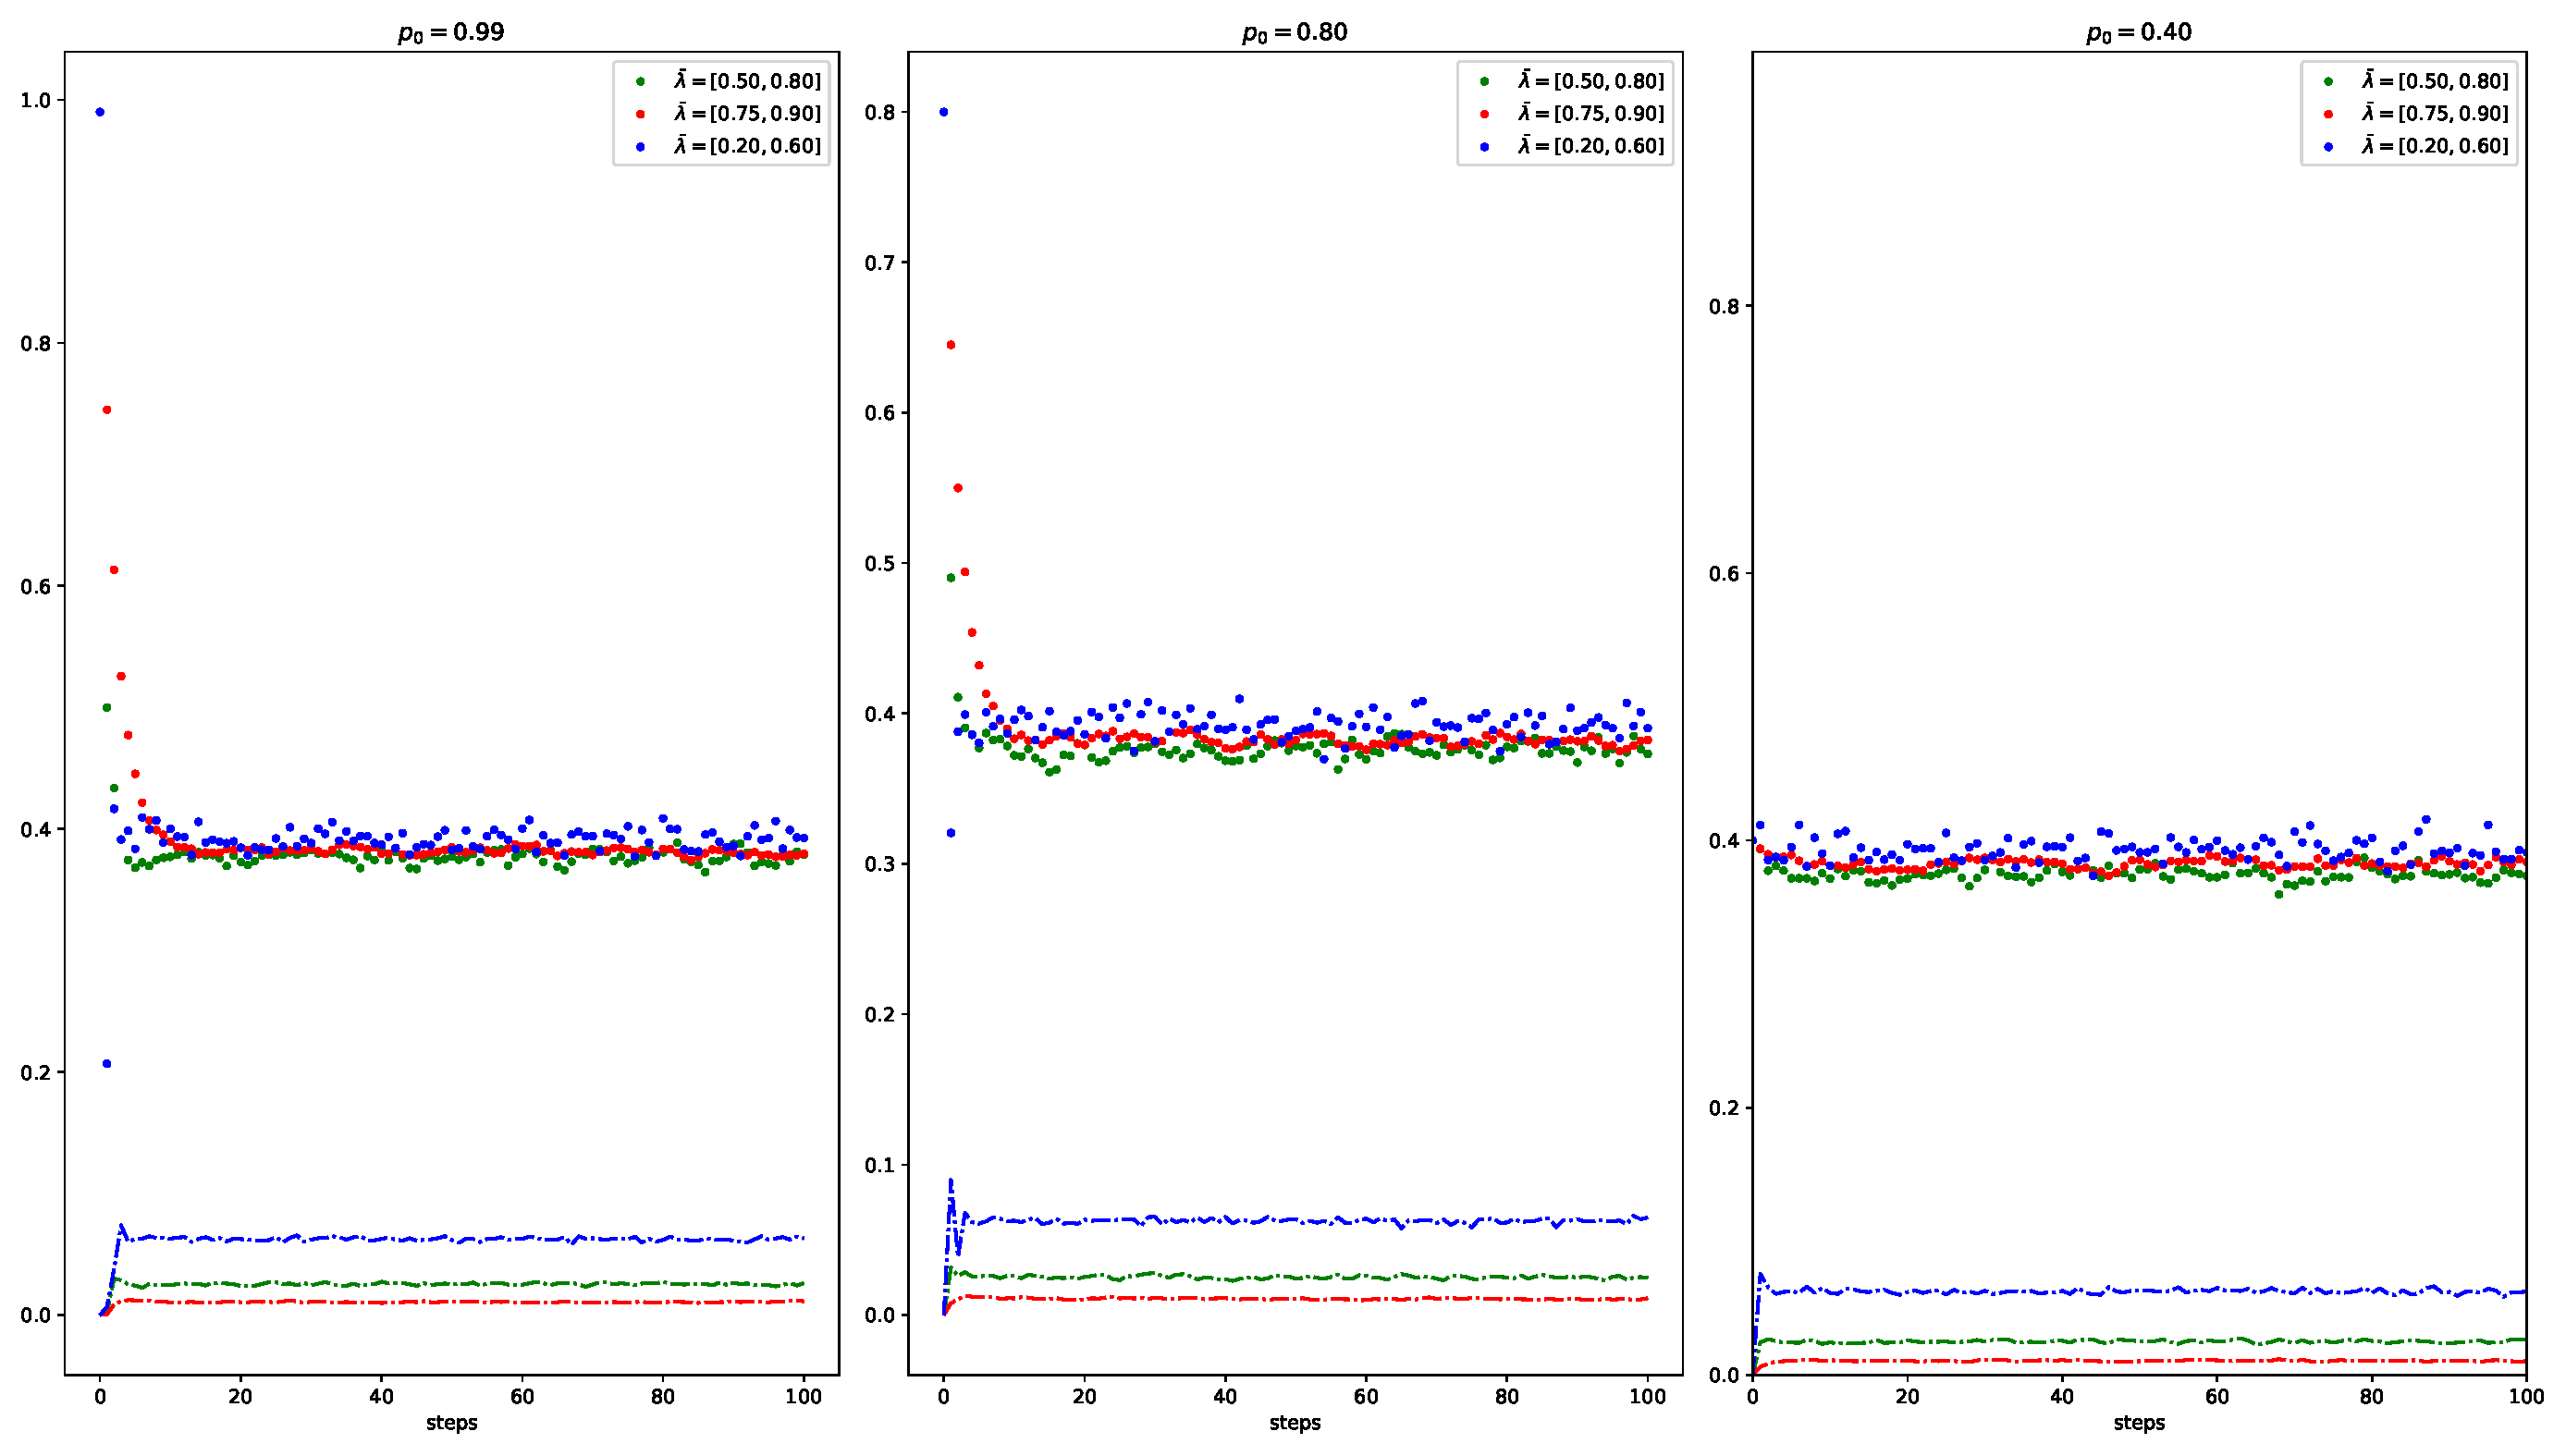
\includegraphics[width=1\textwidth]{../simulations/e_probability_1000_walks_100_steps_type_success_punished_two_lambdas}
\caption{\label{fig:Development-punish2l}The development of the observed average
transition probability (dotted, upper part of the figure) of a \emph{two-parameter success
punishing} version of the random walk and its variance (dot-dashed lines, lower part of the figure). The values
were computed from 1000 simulated realizations of each parameter
combination.}
 \end{center}
\end{figure}


\subsection{Other alternatives}

The presented model of a random walk can be further developed and
more versions can be derived and described. These variants include,
but are not limited to, a multidimensional walk (with either one or multiple
$\lambda$ parameters, \emph{success rewarding} or \emph{success
punishing}), a walk with the transition probability explicitly dependent
on more than the last step, i.e. $P_{t}(k)\sim P_{t}(X_{t},\,X_{t-1},\dots,X_{t-(k-1)})$,
or a walk with $\lambda$ parameter not constant, but a function
of the time $t$, i.e. $P_{t}(\lambda(t)$). Detailed properties of
such walks together with their possible applications on real life
problems will by subject of a further study.

\section{Simulations\label{sec:Simulations}}

Testing dataset was generated in order to validate the quality of
the model and its ability to be fitted on a real life problem. The
data generation was performed using the Python programming language
and its package NumPy. Following values of input parameters were chosen.
The memory coefficient values varied in $\lambda\in\{0.5,\,0.8,\,0.9,\,0.99\}$
and similarly the pair of memory coefficients $[\lambda_{0},\,\lambda_{1}]\in\{[0.5,\,0.8],\,[0.1,\,0.5],\,[0.5,\,0.99],\,[0.99,\,0.9]\}$, further denoted as $\tilde{\lambda}$.
The starting transition probability $p_{0}$ was chosen from the set
$P_{0}=\{0.5,\,0.8,\,0.9,\,0.99\}$ and the length of the walk varied in
\textbf{${\color{red}length}\in\{5,\,10,\,50,\,100\}$}. All four described models of the random walk were tested. For each permutation of the
parameters and the model type $100$ walks were generated and considered as $1$ {\color{red}evaluation set}. Further, $100$ such {\color{red}evaluation sets} were generated, which then formed a dataset consisting of $100\cdot100\cdot4^4=2\,560\,000$ random walks. 

Four different fitting tasks were performed on each of the $100$ {\color{red}evaluation sets}, generating $100$ different estimates for each walk configuration. The tasks were:

\begin{itemize}
\item find $\tilde{\lambda}$ with known $p_{0}$ and model type,
\item find $p_{0}$ with known $\tilde{\lambda}$ and model type,
\item find $p_{0}$ and $\tilde{\lambda}$ with known model type,
\item find model type without any prior knowledge.
\end{itemize}

The first three tasks consist of estimation of parameters and were based on the maximum likelihood estimate (MLE) \cite{rossi2018mathematical}. The evaluation of the likelihood function for given parameters is easy, however the computation of the log-likelihood derivatives is hardly tractable. The ML estimates were therefore obtained using numerical methods with the help of the Python programming language and its scientific package SciPy. The Akaike Information Criterion $AIC=2k-2ln(\hat{L})$, where $k$ is the number of model parameters and $\hat{L}$ is the maximal likelihood, was then used for the last task.

\begin{table} \color{red}
\begin{centering}
{\caption{\label{tab:Fitting-results} The table shows an example of evaluation results.
The first four rows show the results of fitting $\lambda$ or $\lambda_{0}$ with true value $0.5$ (and corresponding $\lambda_{1}=0.8$), known $p_0=0.5$ and walk length $5$, the last four rows the results of the same parameter combination but with walk length $100$.
The mean value and its standard deviation and the median and the corresponding ``percentile'' interval of the 100 evaluation sets are presented.
\emph{SP} stands for \emph{success punishing}, \emph{SR} for \emph{success rewarding}, the number $2$ denotes the model with two $\lambda$ parameters.}}
\begin{tabular}{|c|c|c|c|c|}
\hline
Type & mean & st. dev. & median & percentile \tabularnewline
\hline
SP & 0.505 & 0.043 & 0.504 & $[0.439;0.576]$ \tabularnewline
\hline
SR & 0.502 & 0.033 & 0.503 & $[0.451;0.549]$ \tabularnewline
\hline
SP2 & 0.505 & 0.060 & 0.501 & $[0.399;0.606]$ \tabularnewline
\hline
SR2 & 0.491 & 0.047 & 0.490 & $[0.415;0.564]$ \tabularnewline
\hline
\hline
SP & 0.499 & 0.008 & 0.499 & $[0.484;0.511]$ \tabularnewline
\hline
SR & - & - & - & - \tabularnewline
\hline
SP2 & 0.502 & 0.012 & 0.502 & $[0.478;0.521]$ \tabularnewline
\hline
SR2 & 0.498 & 0.026 & 0.501 & $[0.452;0.535]$ \tabularnewline
\hline
\end{tabular}
\par\end{centering}
\end{table}

To evaluate the quality of the parameter fitting results four different {\color{red}evaluation} criteria were tested. First, the standard $\color{red}(1-\alpha)$ two-sided confidence interval around the mean was constructed and the test was positive if the true parameter value was in that interval. Second, the $\frac{{\color{red}100}\alpha}{2}-th$ and ${\color{red}100(1}-\frac{\alpha}{2})-th$ percentile were chosen as a lower and upper bounds of a ``percentile'' interval and again the test was positive if the true parameter value fell within the interval. {\color{red}For the last two criteria}, a ``proximity'' interval was constructed based on the true parameter value {\color{red}$\omega$ as $[\omega-\frac{\alpha}{2}\omega,\,\omega+\frac{\alpha}{2}\omega]$} and it was tested whether {\color{yellow}the mean} fitted parameter value and {\color{yellow} the median} fitted parameter value fell into that interval. To evaluate the quality of model type estimation simply the proportion of correctly predicted model types for the given walk configuration was computed.

Together there were $1024$ different fitting setups. The overall performance of the fitting is rather satisfying with average success rate of the tests at about $80\%$ (for $\alpha={\color{red}0.1})$. As expected, the less parameters there were to estimate the better the results. Longer walks show better results when finding the coefficients $\tilde{\lambda}$ while the performance in finding correct $p_0$ seems independent on the walk's length. This is not surprising as the parameter $p_0$ affects mostly the first few steps of the walk, while $\tilde{\lambda}$ play their role thorough the entire course of the walk. An example of the results of parameters estimation (tasks 1-3) can be seen in Table \ref{tab:Fitting-results}. Some results of the model type identification using the AIC (task 4) can be observed in Table \ref{tab:Fitting-results-model}. 

For the \emph{success rewarding} version of the model the fitting results were sometimes unsatisfactory and the optimization algorithm often provided a very bad estimate or did not converge at all. The reason for such behavior can be explained be the difference between the theoretical model (where $0<{\color{red}P_t}<1$, {\color{red}for all} $t$) and its representation in computer simulation, where the limited precision handles values very close to $1$ or $0$ as equal to them. This is especially true for walks with more steps. Handling of such unwanted behavior will be subject of further research. 

Full results of all {\color{red}evaluation} setups as well as several values of parameter $\alpha$ can be found in the GitHub repository (see the last paragraph of the paper). 

\begin{table}
\centering{}

{\caption{\label{tab:Fitting-results-model}The table shows the success {\color{red} rate} of model estimation. Model with the lowest value of AIC was selected.}
\begin{tabular}{|c|c|c|c|c|}
\hline
True model & $\tilde{\lambda}$  & $p_0$  & steps & {\color{red}succ. rate} \tabularnewline
\hline
SR & $0.5$  & $0.5$  & 50 & 0.85 \tabularnewline
\hline
SP & $0.5$  & $0.8$  & 5 & 0.88 \tabularnewline
\hline
SR2 & $[0.5,0.8]$  & $0.9$  & 5 & 0.96 \tabularnewline
\hline
SP2 & $[0.99,0.9]$  & $0.99$  & 50 & 0.99 \tabularnewline
\hline
\end{tabular}
}
\end{table}

\section{Conclusion\label{sec:Conclusion}}

This work follows up on the recent results on random walks with varying
probabilities. It describes and proves certain properties of such
a walk, other properties have been studied with the help of numerical
methods. The study also shows the results of the maximum likelihood
and $AIC$ based estimations of model parameters and types using optimization
procedures. The method has been successfully tested on a set of randomly
generated data. The presented model has also many possible uses in
real life applications. Such a type of random walk describes especially
well processes where either a single or just a small number of events
can significantly affect the future development of the process. Such
processes can be found in reliability analysis, medical as well as
econometric studies, and very often in sports modeling. The authors
recently published a study where the \emph{\color{blue}success rewarding} model was applied
to predict the \emph{in-play} development of a Grand Slam tennis matches
with compelling results when used for live betting against a bookmaker
\cite{ja2019imam}.

The source code containing all functionality mentioned in this article
is freely available as open source at
GitHub (https://github.com/tomaskourim/amistat2019).


\bibliographystyle{plain}
\bibliography{doktknih}

{\small
{\em Authors' addresses}:
{\em Tom\'{a}\v{s} Kou\v{r}im}, Faculty of Nuclear Sciences and Physical Engineering, Czech Technical University in Prague,
Czech Republic
 e-mail: \texttt{kourim@\allowbreak outlook.com}.
{\em Petr Volf}, Institute of Information Theory and Automation, Academy of Sciences of the Czech Republic, Prague
 e-mail: \texttt{volf@\allowbreak utia.cas.cz}.
}


\end{document}
